%%---------------------------------------------------------------------------%%
%% SIAM CSE 2015 Presentation
%%---------------------------------------------------------------------------%%

\documentclass{beamer}
\usefonttheme[onlymath]{serif}
\usepackage{colortbl}
\usepackage{longtable,ltcaption,array}
%% The amssymb package provides various useful mathematical symbols
\usepackage{amssymb}
%% The amsthm package provides extended theorem environments
\usepackage{amsthm} \usepackage{amsmath} \usepackage{tmadd,tmath}
\usepackage{booktabs}
\usepackage{multirow}
\usepackage{caption}
\usepackage[labelformat=empty]{subcaption}
\usepackage{tabularx}

%%---------------------------------------------------------------------------%%
%% THEME SETUP

\usetheme{CambridgeUS}
\usecolortheme{spruce}

%%---------------------------------------------------------------------------%%
%% SETUP STUFF
%%---------------------------------------------------------------------------%%

\logo{
\includegraphics[width=2cm]{new_logo}}

\setbeamercolor{item}{fg=MSUgreen}
%\setbeamertemplate{headline}{}
\setbeamertemplate{navigation symbols}{}

\newlength{\DUtablewidth} % internal use in tables

%%---------------------------------------------------------------------------%%
%% MATH STUFF
%%---------------------------------------------------------------------------%%

\newcommand{\Pn}{\textit{P}$\negthinspace_N$}
\newcommand{\SPn}{\textit{SP}$\negthinspace_N$}

\newcommand{\vOmega}{\ensuremath{\ve{\Omega}}}
\newcommand{\hOmega}{\ensuremath{\hat{\ve{\Omega}}}}

\newcommand{\sigs}{\ensuremath{\sigma_{\text{s}}}}
\newcommand{\sigf}{\ensuremath{\sigma_{\text{f}}}}
\newcommand{\sigsm}{\ensuremath{\sigma_{\text{s}m}}}
\newcommand{\sigsn}{\ensuremath{\sigma_{\text{s}n}}}

\newcommand{\phig}{\ensuremath{\Phi}}
\newcommand{\Sigmag}{\ensuremath{\mathbf{\Sigma}}}
\newcommand{\Dg}{\ensuremath{\mathbb{D}}}
\newcommand{\Fg}{\ensuremath{\mathbb{F}}}
\newcommand{\Qg}{\ensuremath{\mathbb{Q}}}
\newcommand{\ug}{\ensuremath{\mathbb{U}}}
\newcommand{\Ag}{\ensuremath{\mathbb{A}}}
\newcommand{\Bg}{\ensuremath{\mathbb{B}}}
\newcommand{\Cg}{\ensuremath{\mathbb{C}}}
\newcommand{\Jg}{\ensuremath{\mathbb{J}}}
\newcommand{\sg}{\ensuremath{\mathbb{S}}}

\newcommand{\aphig}{\ensuremath{\Phi^{\dagger}}}
\newcommand{\aSigmag}{\ensuremath{\mathbf{\Sigma}^{\dagger}}}

\newcommand{\apsi}[1]{\ensuremath{\psi^{\dagger\,#1}}}
\newcommand{\aphi}[1]{\ensuremath{\phi^{\dagger\,#1}}}
\newcommand{\aq}[1]{\ensuremath{q^{\dagger\,#1}}}
\newcommand{\ak}{\ensuremath{k^{\dagger}}}

\newcommand{\normal}{\ensuremath{\hat{\ve{n}}}}

% Phantom minus sign for helping with alignment of matrices
\newcommand{\phmin}{\ensuremath{\phantom{-}}}

\DeclareMathOperator{\diag}{diag}


%%---------------------------------------------------------------------------%%
%% TITLE

\title[Parallel Monte Carlo Solvers]{Parallel Algorithms for Monte Carlo
  Linear Solvers}
\author[Slattery, Hamilton, Evans]{Stuart Slattery
  \\ Steven Hamilton \\ Tom Evans (PI) }
\date[3/17/15]{March 17, 2015}
\institute[]{\small Oak Ridge National Laboratory}
\titlegraphic{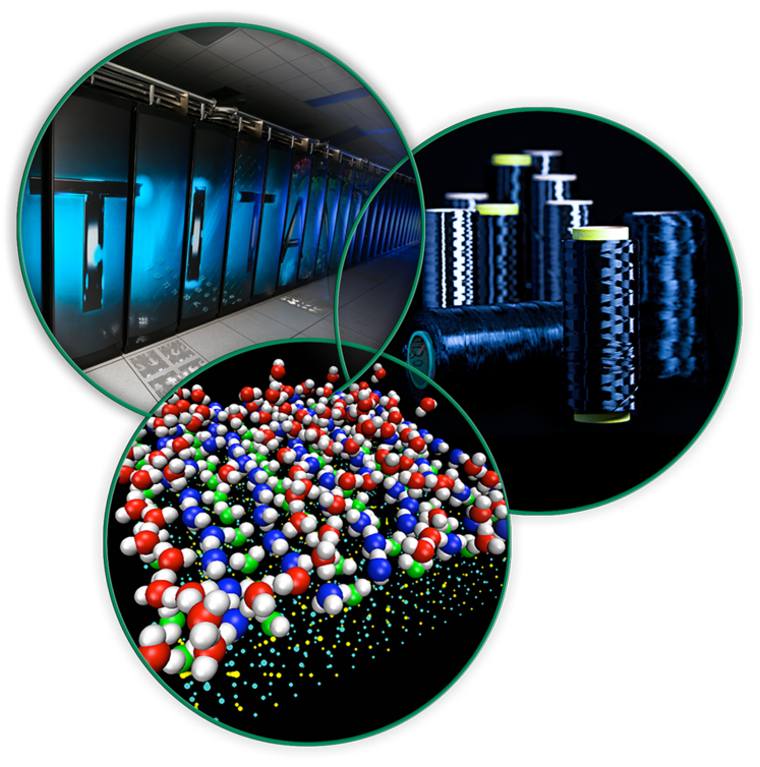
\includegraphics[width=1.5in]{ORNL_Balls.pdf}}

\defbeamertemplate{footline}{titlefoot}{
    \vspace{-0.5cm}
    \hspace*{0.25cm}
    
\includegraphics[width=2cm]{doe_logo}
    \hfill
    
\includegraphics[width=3.25cm]{WordMarkLeaf}
    \hspace*{0.5cm}
}

\setbeamertemplate{title page}
{
  \begin{tabular}{cr}
    \begin{minipage}{4.7cm}
      {\bf \Large\textcolor{MSUgreen}{\inserttitle}}\\

      \vspace{2\baselineskip}
      \insertauthor\\

      \insertinstitute\\

      \insertdate
    \end{minipage}
    &
    \begin{minipage}{5cm}
      \raggedright
      \vspace{-0.75cm}
      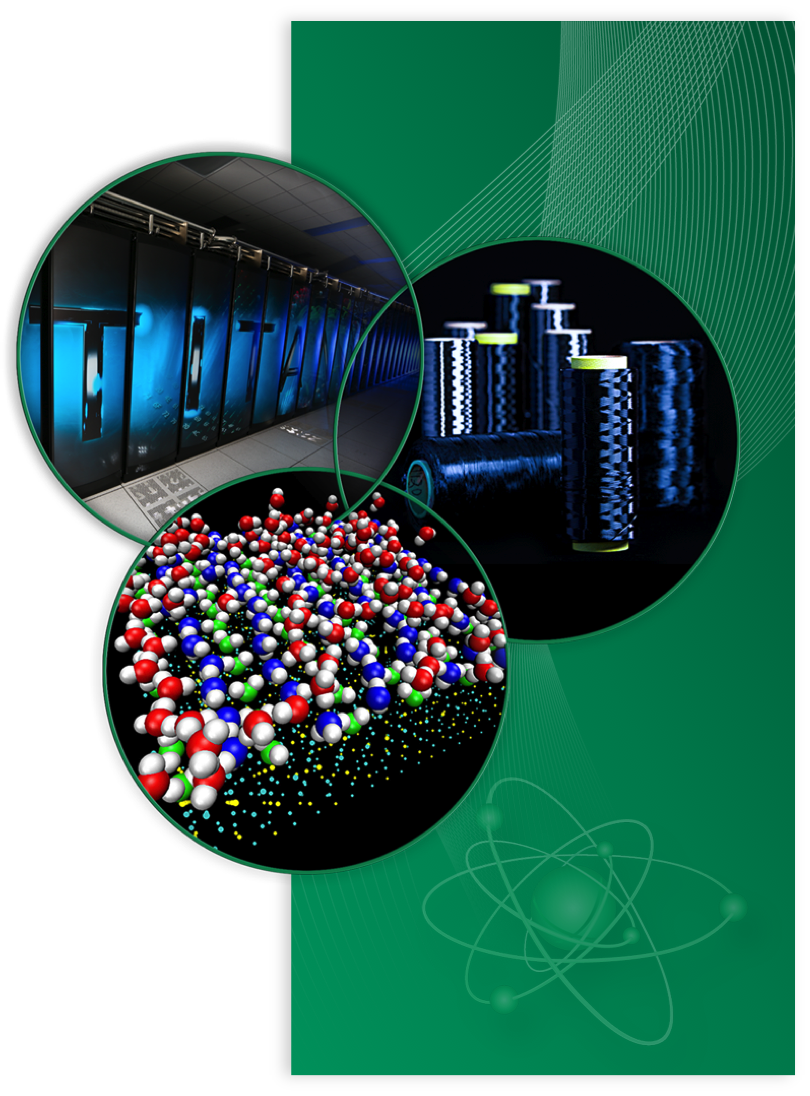
\includegraphics[height=9.8cm]{combined_background}
    \end{minipage}
  \end{tabular}
}

%%---------------------------------------------------------------------------%%
\begin{document}

%%---------------------------------------------------------------------------%%

{
\setbeamertemplate{logo}{}
\setbeamertemplate{footline}[titlefoot]
\begin{frame}
\titlepage
\end{frame}
}

%%---------------------------------------------------------------------------%%
\begin{frame}{Acknowledgments}

  This material is based upon work supported by the U.S. Department of
  Energy, Office of Science, Advanced Scientific Computing Research
  program.

  \vfill

  This research used resources of the Oak Ridge Leadership Computing
  Facility at the Oak Ridge National Laboratory, which is supported by the
  Office of Science of the U.S. Department of Energy under Contract No.
  DE-AC05-00OR22725.

\end{frame}

%%---------------------------------------------------------------------------%%
\frame{\tableofcontents}

%%---------------------------------------------------------------------------%%
\section{Motivation}
%%---------------------------------------------------------------------------%%
\begin{frame}{Motivation}

  \begin{itemize}
    \small
  \item As we move towards exascale computing, the rate of errors is expected
    to increase dramatically
    \vfill
  \item Algorithms need to not only have increased concurrency/scalability
    but have the ability to recover from hardware faults
    \vfill
  \item Two basic strategies:
    \vfill
    \begin{enumerate}
    \item Start with current ``state of the art'' methods and make
      incremental modifications to improve scalability and fault
      tolerance
      \begin{itemize}
      \item Many efforts are heading in this direction, attempting
        to find additional concurrency to exploit
      \end{itemize}
    \item Start with methods having natural scalability and resiliency
      aspects and work at improving performance (e.g. Monte Carlo)
      \begin{itemize}
      \item Soft failures introduce an additional stochastic error
        component
      \item Hard failures potentially mitigated by replication
      \item Concurrency enabled by several levels of parallelism
      \end{itemize}
    \end{enumerate}
  \end{itemize}

\end{frame}

%%---------------------------------------------------------------------------%%
\section{Monte Carlo Methods}

%%---------------------------------------------------------------------------%%
\begin{frame}{Monte Carlo for Linear Systems}
  \begin{itemize}
    \item Suppose we want to solve $\mathbf{Ax}=\mathbf{b}$
    \vfill
    \item If $\rho(\mathbf{I-A})<1$, we can write the solution using the
      Neumann series
      \begin{equation*}
        \mathbf{x} = \sum_{n=0}^{\infty} (\mathbf{I-A})^n \mathbf{b}
         = \sum_{n=0}^{\infty} \mathbf{H}^n \mathbf{b}
      \end{equation*}
      where $\mathbf{H} \equiv ( \mathbf{I-A} )$ is the Richardson
      iteration matrix 
      \vfill
    \item Build the Neumann series stochastically
  \end{itemize}

  \[
  x_i = \sum_{k=0}^{\infty}\sum_{i_1}^{N}\sum_{i_2}^{N}\ldots
  \sum_{i_k}^{N}h_{i,i_1}h_{i_1,i_2}\ldots h_{i_{k-1},i_k}b_{i_k}
  \]

  \begin{itemize}
  \item Define a sequence of state transitions
  \end{itemize}
  \vspace*{-0.1in}
  \[
  \nu = i \rightarrow i_1 \rightarrow \cdots \rightarrow i_{k-1}
  \rightarrow i_{k}
  \]

\end{frame}

%%---------------------------------------------------------------------------%%
\begin{frame}{Forward Monte Carlo}
\begin{itemize}
  \item Choose a row-stochastic matrix $\mathbf{P}$ and weight matrix
    $\mathbf{W}$ such that $\mathbf{H} = \mathbf{P} \circ \mathbf{W}$
  \item Typical choice (Monte Carlo Almost-Optimal):
    \begin{equation*}
      \mathbf{P}_{ij} = \frac{| \mathbf{H}_{ij}| }
      {\sum_{j=1}^{N} | \mathbf{H}_{ij} | }
    \end{equation*}
  \item To compute solution component $\mathbf{x}_i$:
    \begin{itemize}
      \item Start a history in state $i$ (with initial weight of 1)
      \item Transition to new state $j$ based probabilities determined by
        $\mathbf{P}_i$
      \item Modify history weight based on corresponding entry in
        $\mathbf{W}_{ij}$
      \item Add contribution to $\mathbf{x}_i$ based on current history weight
        and value of $\mathbf{b}_j$
    \end{itemize}
  \item A given random walk can only contribute to a single component of
    the solution vector with $\mathbf{x} \approx \mathbf{M_{MC}} \mathbf{b}$
\end{itemize}
\end{frame}

%%---------------------------------------------------------------------------%%
\begin{frame}{Sampling Example (Forward Monte Carlo)}
  \begin{itemize}
    \item Suppose
  \begin{equation*}
    \mathbf{A} = \begin{bmatrix}
      \phmin 1.0 & -0.2 & -0.6 \\
      -0.4 & \phmin 1.0 & -0.4 \\
      -0.1 & -0.4 & \phmin 1.0 \end{bmatrix} \to
    \mathbf{H} \equiv (\mathbf{I-A}) = \begin{bmatrix}
       0.0 &  0.2 &  0.6 \\
       0.4 &  0.0 &  0.4 \\
       0.1 &  0.4 &  0.0 \end{bmatrix}
  \end{equation*}
    then
  \begin{equation*}
    \mathbf{P} = \begin{bmatrix}
       0.0 & 0.25 & 0.75 \\
       0.5 &  0.0 & 0.5 \\
       0.2 &  0.8 & 0.0 \end{bmatrix}, \quad
    \mathbf{W} = \begin{bmatrix}
       0.0 &  0.8 &  0.8 \\
       0.8 &  0.0 &  0.8 \\
       0.5 &  0.5 &  0.0 \end{bmatrix}
  \end{equation*}
    \vfill
    \item If a history is started in state $3$, there is a $20\%$ chance of
      it transitioning to state $1$ and an $80\%$ chance of moving to state
      $2$
  \end{itemize}
\end{frame}

%%---------------------------------------------------------------------------%%
\begin{frame}{Solving the Heat Equation: Forward Method}

  \begin{figure}[h!]
    \begin{center}
      \includegraphics<1>[width=3.75in]{direct_1.png}
      \includegraphics<2>[width=3.75in]{direct_10.png}
      \includegraphics<3>[width=3.75in]{direct_100.png}
      \includegraphics<4>[width=3.75in]{direct_1000.png}
    \end{center}
    \caption{
      \only<1>{\sn{2.5}{3} total histories.}
      \only<2>{\sn{2.5}{4} total histories.}
      \only<3>{\sn{2.5}{5} total histories.}
      \only<4>{\sn{2.5}{6} total histories.}
    }
  \end{figure}

\end{frame}

%%---------------------------------------------------------------------------%%
\section{Domain Decomposition and Replication}

%%---------------------------------------------------------------------------%%
\begin{frame}{Domain Decomposed Monte Carlo}

  \begin{columns}
    \begin{column}{0.5\textwidth}
      \begin{itemize}
      \item Each parallel process owns a piece of the domain (linear
        system)
        \bigskip
      \item Random walks must be transported between adjacent domains
        through parallel communication
        \bigskip
      \item Domain decomposition determined by the input system
        \bigskip
      \item Load balancing not yet addressed
      \end{itemize}
    \end{column}

    \begin{column}{0.5\textwidth}
      \begin{figure}[htpb!]
        \begin{center}
          \scalebox{0.75}{ \input{ddnu_example.pdftex_t} }
        \end{center}
        \caption{\small Domain decomposition example illustrating
          how domain-to-domain transport creates communication costs.}
      \end{figure}
    \end{column}
  \end{columns}

\end{frame}

%%---------------------------------------------------------------------------%%
\begin{frame}{Asynchronous Monte Carlo Transport Kernel}

  \begin{columns}

    \begin{column}{0.5\textwidth}
      \vspace{-0.1in}
      \small
      \begin{itemize}
      \item General extension of the Milagro algorithm (LANL)
      \item Asynchronous nearest neighbor communication of histories
      \item System-tunable communication parameters of buffer size and check
        frequency (performance impact)
      \item Need an asynchronous strategy for exiting the transport loop
        without a collective (running sum)
      \end{itemize}

      \vspace{-0.15in}
      \begin{figure}[htpb!]
        \begin{center}
          \scalebox{0.4}{ \input{domain_to_domain.pdftex_t} }
        \end{center}
      \end{figure}

    \end{column}

    \begin{column}{0.5\textwidth}

      \vspace{-0.25in}
      \begin{figure}[htpb!]
        \begin{center}
          \scalebox{0.825}{ \input{transport_loop.pdftex_t} }
        \end{center}
      \end{figure}

    \end{column}

  \end{columns}

\end{frame}

%%---------------------------------------------------------------------------%%
\begin{frame}{Exiting the Transport Loop without Collectives}

  \vspace{-0.2in}

  \begin{figure}[htpb!]
    \begin{center}
      \scalebox{0.35}{ \input{master_comm_tree.pdftex_t} }
    \end{center}
    \caption{Master/Slave}
  \end{figure}

  \begin{columns}

    \begin{column}{0.5\textwidth}
      \vspace{-0.75in}
      \begin{figure}[htpb!]
        \begin{center}
          \scalebox{0.4}{ \input{binary_comm_tree.pdftex_t} }
        \end{center}
        \caption{Binary Tree}
      \end{figure}

    \end{column}

    \begin{column}{0.5\textwidth}

      \vspace{-0.55in}
      
      \begin{figure}[t!]
        \begin{center}
          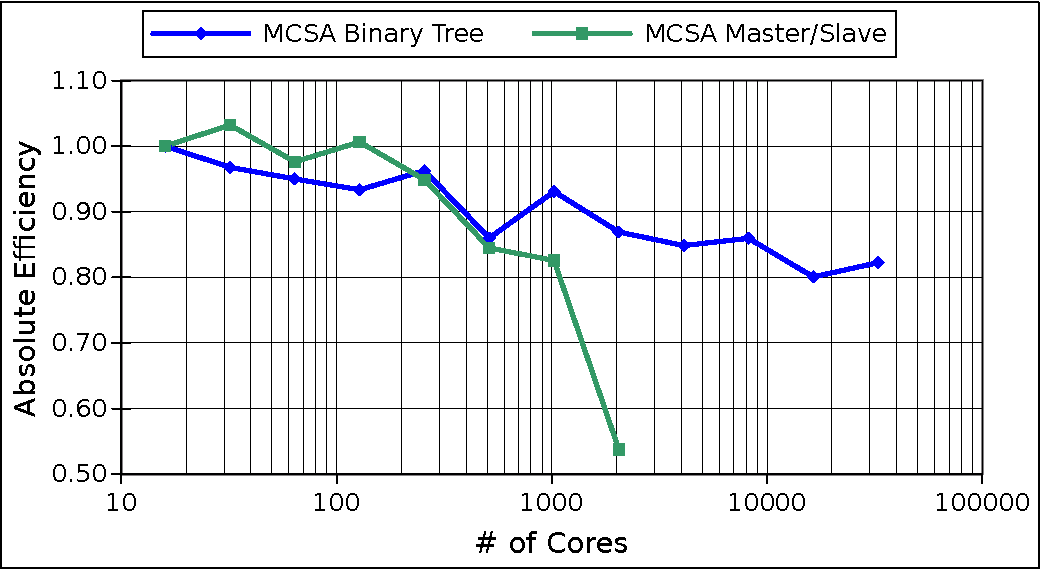
\includegraphics[width=0.99\textwidth]{titan_weak_bvsm.pdf}
        \end{center}
        \caption{Weak scaling absolute efficiency}
        \label{fig:titan_weak_bvsm}
      \end{figure}

    \end{column}

  \end{columns}

\end{frame}

%%---------------------------------------------------------------------------%%
\begin{frame}{Replication}

  \vspace{-0.1in}
  
  Different batches of Monte Carlo samples can be combined in summation via
  superposition if they have different random number streams. For two
  different batches:

  \[
  \mathbf{M_{MC}} \mathbf{x} =
  \frac{1}{2}(\mathbf{M_1}+\mathbf{M_2})\mathbf{x} 
  \]

  Consider each of these batches independent \textit{subsets} of a Monte Carlo
  operator where now the operator can be formed as a general additive
  decomposition of $N_S$ subsets: 

  \[
  \mathbf{M_{MC}} = \frac{1}{N_S}\sum_{n=1}^{N_s}{\mathbf{M_n}}
  \]

  We replicate the linear problem and form each subset on a different group of
  parallel processes. Applying the subsets to a vector requires an AllReduce
  to form the sum. Each subset is domain decomposed.
  
\end{frame}

%%---------------------------------------------------------------------------%%
\section{Scaling Studies}

%%---------------------------------------------------------------------------%%
\begin{frame}{Parallel Test - Simplified $P_N$ ($SP_N$) Assembly Problem}
\small
\begin{columns}
  
    \begin{column}{0.55\textwidth}

      \vspace{-0.2in}
      \begin{figure}
        \centering
        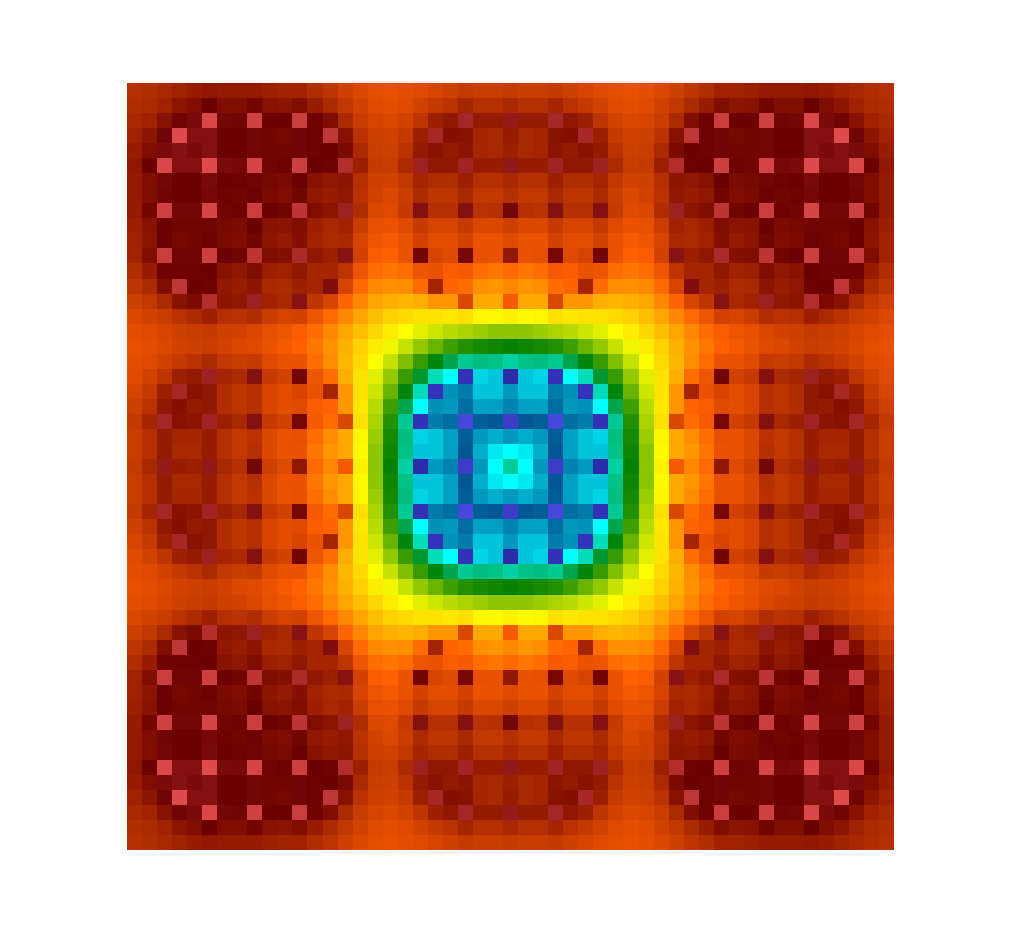
\includegraphics[width=2.0in]{prob4}
        \vspace{-0.2in}
        \caption{$SP_N$ solution example}
      \end{figure}

      \vspace{-0.1in}
      
      The ($SP_N$) equations are an approximation to the Boltzmann neutron
      transport equation used to simulate nuclear reactors

      \vspace{-0.2in}
      
      \[
        \small
        -\nabla \cdot \mathbb{D}_n \nabla \mathbb{U}_n + \sum_{m=1}^4
        \mathbb{A}_{nm} \mathbb{U}_m = \frac{1}{k} \sum_{m=1}^4
        \mathbb{F}_{nm} \mathbb{U}_m
      \]

    \end{column}

    \begin{column}{0.45\textwidth}
      Scaling problem -- $1 \times 1$ to $17 \times 17$ array of fuel
      assemblies with 289 pins each resolved by a $2 \times 2$ spatial mesh
      and 200 axial zones

      \vfill
      
      \begin{itemize}
      \item 7 energy groups, 1 angular moment, 1.6M to 273.5M degrees of
        freedom
      \item 64 to 10,800 computational cores via domain decomposition
      \item We are usually interested in solving generalized eigenvalue
        problem - we use the operator from these problems to test the kernel
        scaling 
      \end{itemize}
    \end{column}
    
  \end{columns}

\end{frame}

%%---------------------------------------------------------------------------%%
\begin{frame}{Monte Carlo Communication Parameters}

  \vspace{-0.3in}
  
  \begin{table}[htb!]
    \begin{center}
      \small
      \begin{tabular}{rr|rrrr}
        \toprule
        \multicolumn{6}{r}{Message Check Frequency} \\
        \multicolumn{1}{r}{} &
        \multicolumn{1}{r}{} &
        \multicolumn{1}{r}{\textbf{128}} &
        \multicolumn{1}{r}{\textbf{256}} &
        \multicolumn{1}{r}{\textbf{512}} &
        \multicolumn{1}{r}{\textbf{1\,024}}
        \\ \midrule
        \multirow{7}{*}{{Message Buffer Size}}
        %%
        & \textbf{256}	& 1.054	& 1.061	& 1.076	& 1.076 \\
        & \textbf{512}	& 1.103	& 1.146	& 1.211	& \framebox[1.1\width]{1.270} \\
        & \textbf{1\,024}	& 1.062	& 1.088	& 1.133	& 1.176 \\
        & \textbf{2\,048}	& 1.030	& 1.042	& 1.072	& 1.107 \\
        & \textbf{4\,096}	& 1.010	& 1.012	& 1.025	& 1.050 \\
        & \textbf{8\,192}	& 1.001	& \framebox[1.1\width]{1.000}	& 1.008	& 1.018 \\
        & \textbf{16\,384}	& 1.017	& 1.003	& 1.010	& 1.009 \\
        %%
        \bottomrule
      \end{tabular}
    \end{center}
  \end{table} 

  \vspace{-0.2in}
  
  \begin{itemize}
    \small
  \item OLCF Eos: 736-node Cray XC30, Intel® Xeon® E5-2670, 11,776
    cores, 47 TB memory, Cray Aries interconnect
  \item 64 cores, 1.6M DOFs, history length of 15, 3 histories per DOF
  \item 27\% decrease in runtime observed for bad parameter choices
  \item Worth the time to do this parameter study when running on new
    hardware
  \end{itemize}
  
\end{frame}

%%---------------------------------------------------------------------------%%
\begin{frame}{Domain Decomposition Scaling}

  \vspace{-0.2in}
  
  \begin{table}[htb!]
    \tiny
    \begin{center}
      \begin{tabular}{rrrrrrr}
        \toprule
        \multicolumn{1}{r}{Cores} &
        \multicolumn{1}{r}{DOFs} &
        \multicolumn{1}{r}{DOFs/Core} &
        \multicolumn{1}{r}{Time Min (s)} &
        \multicolumn{1}{r}{Time Max (s)} &
        \multicolumn{1}{r}{Time Ave (s)} &
        \multicolumn{1}{r}{Efficiency}
        \\ \midrule
        %%
        256 & 273\,509\,600 & 1\,068\,397 & 515.51 & 515.52 & 515.52 & 1.00 \\
        1\,024 & 273\,509\,600 & 267\,099 & 122.76 & 122.77 & 122.76 & 1.05 \\
        4\,096 & 273\,509\,600 & 66\,775 & 27.96 & 27.97 & 27.96 & 1.15 \\
        7\,744 & 273\,509\,600 & 35\,319 & 17.72 & 17.72 & 17.72 & 0.96 \\
        10\,816 & 273\,509\,600 & 25\,288 & 13.72 & 13.72 & 13.72 & 0.89 \\
        %%
        \bottomrule
      \end{tabular}
    \end{center}
    \vspace{-0.07in}
    \caption{\small Strong Scaling}
  \end{table} 

  \vspace{-0.4in}
  
  \begin{table}[htb!]
    \tiny
    \begin{center}
      \begin{tabular}{rrrrrrr}
        \toprule
        \multicolumn{1}{r}{Cores} &
        \multicolumn{1}{r}{DOFs} &
        \multicolumn{1}{r}{DOFs/Core} &
        \multicolumn{1}{r}{Time Min (s)} &
        \multicolumn{1}{r}{Time Max (s)} &
        \multicolumn{1}{r}{Time Ave (s)} &
        \multicolumn{1}{r}{Efficiency}
        \\ \midrule
        %%
        64 & 1\,618\,400 & 25\,288 & 12.65 & 12.65 & 12.65 & 1.00 \\
        256 & 6\,473\,600 & 25\,288 & 12.86 & 12.86 & 12.86 & 0.98 \\
        1\,024 & 25\,894\,400 & 25\,288 & 14.59 & 14.59 & 14.59 & 0.87 \\
        4\,096 & 103\,577\,600 & 25\,288 & 14.25 & 14.25 & 14.25 & 0.89 \\
        7\,744 & 195\,826\,400 & 25\,288 & 14.75 & 14.78 & 14.75 & 0.86 \\
        10\,816 & 273\,509\,600 & 25\,288 & 13.72 & 13.72 & 13.72 & 0.92 \\
        %
        \bottomrule
      \end{tabular}
    \end{center}
        \vspace{-0.07in}
    \caption{\small Weak Scaling}
  \end{table}

  \vspace{-0.25in}
  
  \begin{itemize}
    \small
  \item Titan Cray XK7 was used with no GPUs - used Eos parameters
  \item Results are consistent with transport literature
  \item History length of 15 and 3 histories per DOF
  \item Consider these effective operator apply times of 15 realizations of
    $\ve{H}$
  \item MC dominates run times in solver applications
  \end{itemize}

\end{frame}

%%---------------------------------------------------------------------------%%
\begin{frame}{Replication Scaling}

  \begin{table}[htb!]
    \tiny
    \begin{center}
      \begin{tabular}{rrrrrrr}
        \toprule
        \multicolumn{1}{r}{Subsets} &
        \multicolumn{1}{r}{Cores} &
        \multicolumn{1}{r}{DOFs} &
        \multicolumn{1}{r}{Time Min (s)} &
        \multicolumn{1}{r}{Time Max (s)} &
        \multicolumn{1}{r}{Time Ave (s)} &
        \multicolumn{1}{r}{Efficiency}
        \\ \midrule
        %%
        1 & 256 & 6\,473\,600 & 12.65 & 12.65 & 12.65 & 1.00 \\
        2 & 512 & 6\,473\,600 & 6.62 & 6.80 & 6.72 & 0.93 \\
        3 & 768 & 6\,473\,600 & 4.50 & 4.73 & 4.66 & 0.89 \\
        4 & 1\,024 & 6\,473\,600 & 3.62 & 3.81 & 3.71 & 0.83 \\
        %
        \bottomrule
      \end{tabular}
    \end{center}
    \caption{\small Fixed algorithmic scaling}
  \end{table}

  \vfill
  
  \begin{itemize}
    \small
  \item Timings are Monte Carlo time plus AllReduce time
  \item 256 cores per subset with domain decomposition
  \item $1/N_S$ samples per subset gives flat algorithmic performance
  \item Two performance issues
    \begin{itemize}
    \item Dividing up samples creates work starvation
    \item AllReduce buffer size is constant regardless of work starvation
    \end{itemize}
  \item Research is needed for a more performant subset combination
  \end{itemize}
  
\end{frame}

%%---------------------------------------------------------------------------%%
\section{Current/Future Work and Conclusions}

%%---------------------------------------------------------------------------%%
\begin{frame}{Current Work - Vectorization and Threading}

  \begin{itemize}
  \item We have implemented a Monte Carlo kernel using the Kokkos threading
    model (Trilinos)
    \begin{itemize}
    \item The kernel supports multi-threaded CPU, GPU, and Xeon Phi
      architectures with a single implementation
    \end{itemize}
    \vfill
  \item Vectorization an area of active research with a focus on heterogeneous
    architectures (Titan and Summit)
    \begin{itemize}
    \item Currently investigating event-based algorithms to enable
      vectorization
    \item Event-based algorithm concepts are based on vectorized Monte Carlo
      algorithms from particle transport
    \end{itemize}
    \vfill
  \item We are exploring an additive-Schwarz formulation to eliminate
    parallel communication in the Monte Carlo kernel
    \vfill
  \item Other threading models will be considered (e.g. HPX)
  \end{itemize}
  
\end{frame}

%%---------------------------------------------------------------------------%%
\begin{frame}{Conclusions and Future Work}
  \begin{itemize}
    \small
  \item Monte Carlo methods offer great potential for both resilient and
    highly parallel solvers
    \begin{itemize}
    \item A fully asynchronous algorithm provides scalability without
      collectives
    \item Replication potentially offers resiliency with some overhead
    \end{itemize}
    \vfill
  \item Extending methods to broader problem areas is a significant
    algorithmic challenge and an attractive area for continued research
    \begin{itemize}
    \item Explicit preconditioners are required for all problems
    \end{itemize}
    \vfill
  \item Performance modeling and resiliency simulations this FY
    \begin{itemize}
    \item Fault injection studies using the xSim simulator
    \end{itemize}
  \end{itemize}
\end{frame}

%%---------------------------------------------------------------------------%%
\end{document}
%%---------------------------------------------------------------------------%%

%%---------------------------------------------------------------------------%%
%% end of pres.tex
%%---------------------------------------------------------------------------%%
